% /*==========================================================================================*\
% **                        _           _ _   _     _  _         _                            **
% **                       | |__  _   _/ | |_| |__ | || |  _ __ | |__                         **
% **                       | '_ \| | | | | __| '_ \| || |_| '_ \| '_ \                        **
% **                       | |_) | |_| | | |_| | | |__   _| | | | | | |                       **
% **                       |_.__/ \__,_|_|\__|_| |_|  |_| |_| |_|_| |_|                       **
% \*==========================================================================================*/
% 
%   Invitation to HUST 2024 Graduation Ceremony | Vietnamese Version
%   Author: @bu1th4nh (Bùi Tiến Thành)
%   Date: 2024-04-30 23:57:00
%   URL: https://github.com/bu1th4nh
% 


\documentclass[final,5p,times,twocolumn, 8pt, a4paper]{elsarticle}
\usepackage[utf8]{vietnam}


\usepackage{amssymb}
\usepackage{enumitem}
\usepackage{color}
\usepackage[pdftex, % Sử dụng PDF TeX
bookmarks=true, % Tạo bookmarks trong tập tin PDF
colorlinks=false, % Chữ có màu
pdfencoding=auto, % Tự động điều chỉnh encoding của PDF
unicode=true, % Sử dụng Unicode
pdffitwindow=true, % Fit cho vừa cửa sổ
pdfstartview={FitW}, % Zoom file PDF cho vừa khít với nội dung
pdftoolbar=false, % Ẩn đi tool bar trong PDF viewer
pdfmenubar=false, % Ẩn đi menu bar trong PDF viewer
breaklinks=true % Tránh tràn dòng với liên kết
]{hyperref}



\journal{HUST 2024 Graduation Ceremony}

\begin{document}

    \begin{frontmatter}

        


        \title{Thư mời tham dự Lễ tốt nghiệp 2024 | Phiên bản tiếng Việt}

        \author[1]{Bùi Tiến Thành\corref{cor1}}

        \cortext[cor1]{Corresponding author}
        \ead{bu1th4nh.127@gmail.com}
        \ead[url]{https://github.com/bu1th4nh}




        \affiliation[1]{organization={Khoa Toán - Tin, Đại học Bách khoa Hà Nội},
                    addressline={Số 1 Đại Cồ Việt},
                    city={Quận Hai Bà Trưng, Hà Nội},
                    % postcode={},
                    % state={},
                    country={Việt Nam}}


        \begin{abstract}
            Trong paper này, thư mời tham dự Lễ tốt nghiệp 2024 cho tân cử nhân Bùi Tiến Thành đã được xây dựng. Địa điểm, thời gian, lịch trình và các lưu ý bổ sung đã được trình bày chi tiết. 

        \end{abstract}

        \begin{keyword}
            Tốt nghiệp \sep Đại học Bách khoa Hà Nội \sep Tân cử nhân
        \end{keyword}

    \end{frontmatter}

    %% \linenumbers

    %% main text
    \section{Giới thiệu}
        \par Lễ tốt nghiệp là một sự kiện quan trọng trong cuộc đời của mỗi sinh viên. Đây là dịp để các bạn sinh viên chia tay với trường, với những người bạn, thầy cô đã dạy bảo và cùng nhau tạo nên những kỷ niệm đẹp nhất. Để chuẩn bị cho sự kiện này, một thư mời chính thức đã được xây dựng để mời tất cả các thầy cô, anh/chị/em, bạn bè đến dự, chung vui và lưu lại những bức hình đẹp cùng tân cử nhân Bùi Tiến Thành.


    \section{Phương pháp luận}
        \par Thư mời này được xây dựng bằng LaTeX, với sự chỉnh sửa và bổ sung thông tin cụ thể cho tân cử nhân Bùi Tiến Thành, bao gồm địa điểm, thời gian, lịch trình và các lưu ý bổ sung.

        \subsection{Thời gian}
            \par Lễ tốt nghiệp 2024 sẽ diễn ra vào \textcolor{red}{\textbf{ngày 12 tháng 05 năm 2024}}. Lịch trình chi tiết như sau:
            \begin{enumerate}[label=\roman*)]
                \item Từ 09h30 đến 13h00: Pre-party, tâm sự và chụp ảnh tại khuôn viên Đại học với trang phục thông thường.
                \item Từ 13h00 đến 14h00: Lễ tốt nghiệp tại Hội trường C2.
                \item Từ 14h00 đến 17h30: Tâm sự, chụp ảnh tại khuôn viên Đại học với lễ phục tốt nghiệp.
            \end{enumerate}

        \subsection{Địa điểm}
            \par Lễ tốt nghiệp sẽ diễn ra tại \textcolor{red}{\textbf{Đại học Bách khoa Hà Nội, số 1 Đại Cồ Việt, Quận Hai Bà Trưng}}. Hình \ref{fig:hust} là địa điểm đã được đánh dấu trên Google Earth\footnote[1]{\url{https://earth.google.com/web/}}. Vùng màu \textcolor{red}{đỏ}, viền vàng là khuôn viên Đại học, nơi diễn ra pre-party và chụp ảnh. Marker màu \textcolor{green}{xanh} chỉ địa điểm Hội trường C2, nơi diễn ra lễ tốt nghiệp.
            \begin{figure}
                \centering
                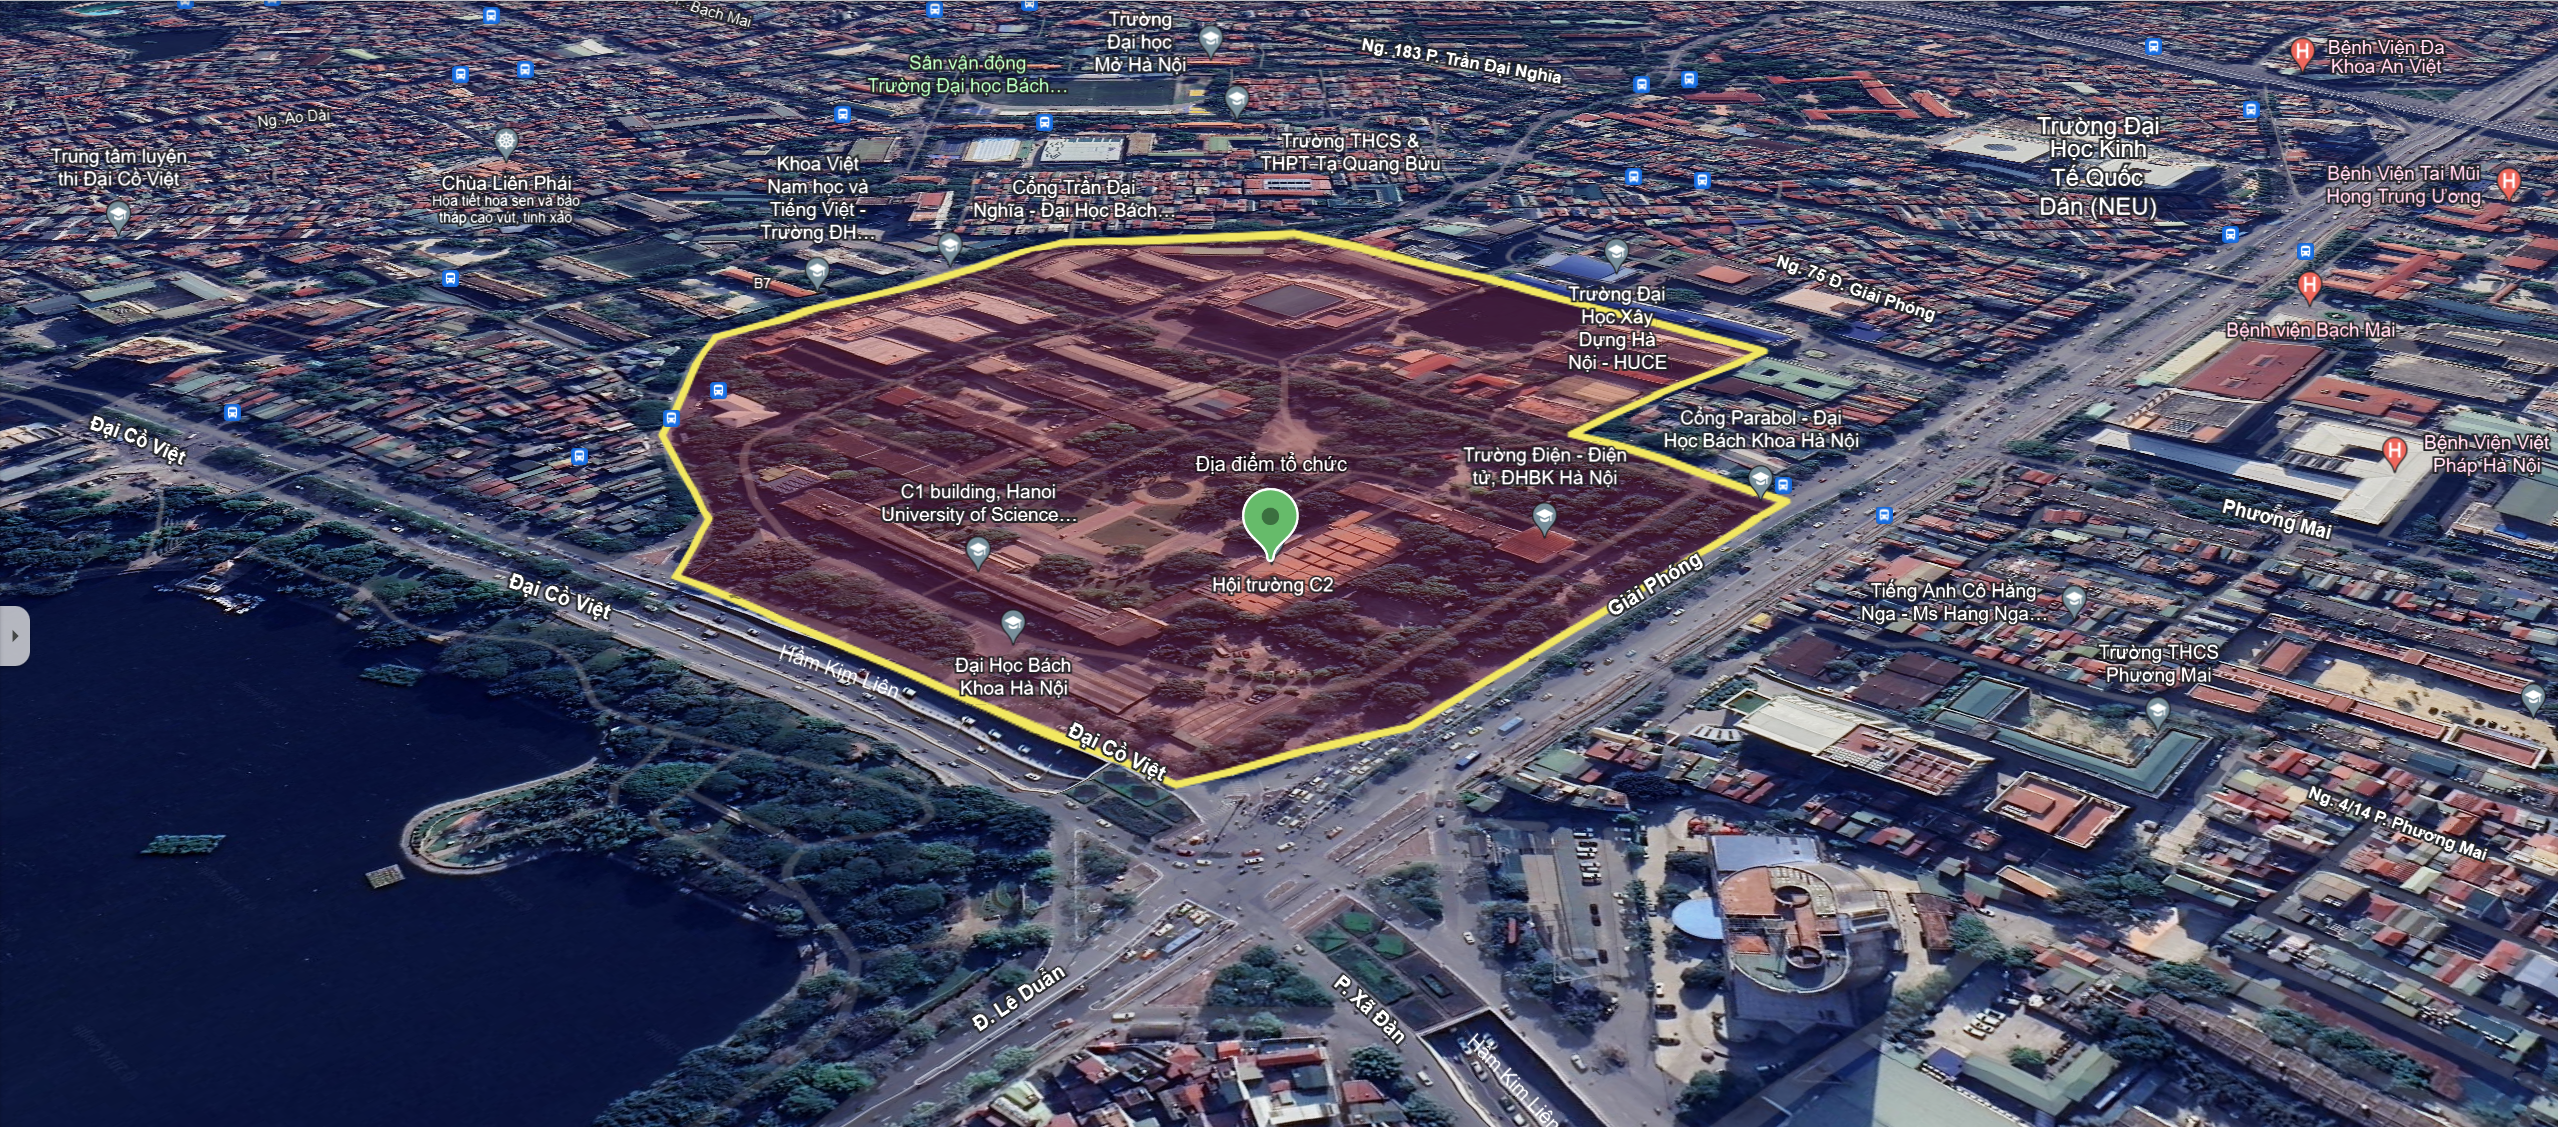
\includegraphics[width=0.45\textwidth]{place.png}
                \caption{Địa điểm tố chức trên Google Earth.}
                \label{fig:hust}
            \end{figure}

        \subsection{Thông tin liên lạc}
            \par Để liên lạc, xin vui lòng liên hệ theo các cách sau:
            \begin{itemize}
                \item \textbf{Facebook/Messenger}: \texttt{\href{https://www.facebook.com/bu1th4nh.127}{facebook.com/bu1th4nh.127}}
                \item \textbf{Số điện thoại}: \texttt{\href{tel:0329436968}{0329436968}}
                \item \textbf{E-mail}: \texttt{\href{mailto:bu1th4nh.127@gmail.com}{bu1th4nh.127@gmail.com}}
            \end{itemize}

        \subsection{Một số lưu ý}
            \par Để chuẩn bị tốt nhất cho sự kiện, cần lưu ý một số điều sau:
            \begin{itemize}
                \item Nên mang theo ô vì thời tiết ngày 12/05 có thể có nắng nóng và có mưa giông vào chiều muộn,
                \item Khuyến nghị mang nước vì ai rồi cũng khát,
                \item Sự tham gia của các bạn là niềm vinh dự và hạnh phúc của tác giả.
            \end{itemize}
    \section{Kết luận}
        \par Lễ tốt nghiệp 2024 của tân cử nhân Bùi Tiến Thành sẽ diễn ra vào ngày 12/05/2024 tại Đại học Bách khoa Hà Nội. Mọi thông tin chi tiết đã được trình bày trong thư mời này. Tác giả xin chân thành cảm ơn và mong nhận được sự tham dự của các bạn/anh/chị/em.

\end{document}
\endinput


% Content and code by bu1th4nh. All rights reserved.
% Powered, inspired and motivated by EDM, Counter-Strike, and Disney Princesses. 
%                                                                                                                                                                                                        
%%%%%%%%%%%%%%%%%%%%%%%%%%%%%%%%%%%%%%%%%%%%%%%%%%%%%%%%%%%%%%%%%%%%%%%%%%%                                ********                                                                                            ⡀⣰    
%%%%%%%%%%%%%%%%%%%%%%%%%%%%%%                                            %                              ***  ******                        ########                                                          ⣰⡿⠃    
%%%%%%%%%%%%%%%%%%%%%%%%%%%%%%                                            %                             ***    ****            #####################                                                         ⣼⣿⣧⠏    
%%%%%%%%%%%%%%%(%%%%%%%%%%%%%%        %%%%  %%%  **   % %  %%   %%%       %                            ****       ##################################                                                        ⣰⣿⠟⠋     
%%%%%%%%%%%%%%#,%%%%%%%%%%%%%%       %%  % %%=%% %%   %=% %./% %          %                           ,****   ######################################                                                        ⣿⡿       
%%%%%%%%%%,,,,,,,,,,,%%%%%%%%%        %%%% %   % %%   % %  %%  %,%%       %             /###########  *****   ######################################                                                       ⣸⣿⡇       
%%%%%%%%%%%%%,,,,,%%%%%%%%%%%%              @              @              %      ###################   *****   #####################################                                         ⣀⣴⣾⣿         ⢰⣿⣿⡇       
%%%%%%%%%%%%,,%%%,,%%%%%%%%%%%                                            %      ###################(  ******  #####################################                                     ⢀⣠⣾⣿⣿⣿⣿⡏         ⣼⣿⣿        
%%%%%%%%%%%%%%%%%%%%%%%%%%%%%%                        %%%/                %      ####################   *****   ####################################                                    ⣠⣿⣿⣿⣿⣿⣿⣿⣤        ⢠⣿⣿⠇        
%%%%%%%%%%%%%%%%%%%%%%%%%%%%%%                    %*,,,,,,%               %      ####################(  **********  .###############################                                   ⣼⣿⣿⣿⣿⣿⣿⣿⣿⣿⣷⣶⡄    ⢀⣾⣿⣿         
%%%%%%%%%%%%%%%%%%%%%%%%%%%%%%                ##,,,,,,%,(%                %      ################## ***  ******     *** .###########################                                  ⣼⣿⣿⣿⣿⣿⣿⣿⣿⣿⣿⣿⣿⣿⠄  ⣤⣾⣿⡟⠁         
%%%%%%%%%%%%%%%%%%%%%%%%%%%%%%            ,%,,,,,,,,,,,/                  %      ################ **     ******        **.##########################                                 ⢠⣿⣿⣿⣿⣿⣿⣿⣿⣿⣿⣿⣿⡏⠁⢀⣴⣾⣿⣿⠏           
%%%%%%%%%%%%%%%%%%%%%%%%%%%%%%         %,,,,,,,%%,,,,,%                   %      ############### **       ******        ** #########################                              ⣀⣀⣴⣿⣿⣿⣿⣿⣿⣿⣿⣿⣿⣿⣿⣿⣧⣴⣿⣿⣿⠿⠁            
%%%%%%%%%%%%%%%%%%%%%%%%%%%%%%     %,,,,,,%#   %,,,,%                     %      ############### **        ******       ** #########################                        ⣀⣤⣶⣿⣿⣿⣿⣿⣿⣿⣿⣿⣿⣿⣿⣿⣿⣿⣿⣿⣿⣿⣿⣿⣿⣿⡏              
%%%%%%%%%%%%%%%%%%%%%%%%%%%%%% %,,,,,%#       #,,,,/                      %      ################ **       ******     *** ##########################                      ⣠⣾⣿⣿⣿⣿⣿⣿⣿⣿⣿⣿⣿⣿⣿⣿⣿⣿⣿⣿⣿⣿⣿⣿⣿⣿⣿⣿⣄              
%%%%%%%%%%%%%%%%%%%%%%%%%%%%*,,,%%           ,,,,%                        %      ##################  ***    *********** ############################                     ⢠⣿⣿⣿⣿⣿⣿⣿⣿⣿⣿⣿⣿⣿⣿⣿⣿⣿⣿⣿⣿⣿⣿⣿⣿⣿⣿⣿⣿⣿⣷⡄            
%%%%%%%%%%%%%%%%%%%%%%%%#,,#%%             %,,,/                          %      #######################    *******  ###############################                     ⣾⣿⣿⣿⠿⣻⣿⣿⣿⣿⣿⣿⣿⣿⣿⣿⣿⣿⣿⣿⣿⣿⣿⣿⣿⣿⣿⣿⣿⣿⣿⡇            
%%%%%%%%%%%%%%%%%%%%%,(%%%%%%%            %,,,%                           %      #########################   ******   ##############################                    ⣸⣿⡿⠉⣠⣾⣿⣿⣿⣿⣿⣿⣿⣿⣿⣿⣿⣿⣿⡿⠟⠉⢿⣿⣿⣿⣿⣿⣿⣿⣿⠟⠁            
%%%%%%%%%%%%%%%%%*%%%%%%%%%%%%           /,,%                             %      ##########################   ******  ##############################                ⠠⣤⣴⣾⡿⠋ ⣼⣿⣿⣿⢟⣿⣿⠏⢰⣿⡿⠟⢻⣿⣿⡿   ⠈⢿⣿⣿⣿⣿⣿⣿⠏              
%%%%%%%%%%%%%%%%%%%%%%%%%%%%%%         /,,,/                              %      ###########################  ******   #############################                      ⣼⣿⣿⡟⠁⣸⡿⠁ ⠘⠋⣀⣴⣿⣿⠟    ⢀⣼⣿⣿⣿⣿⣿⠃               
%%%%%%%%%%%%%%%%%%%%%%%%%%%%%%        %,,%                                %            #####################   ******  #############################                   ⢠⣴⣾⣿⠿⠋ ⠐⠋   ⢀⣾⣿⣿⡿⠋   ⣠⣴⣾⣿⣿⣿⣿⣿⠃                
%%%%%%%%%%%%%%%%%%%%%%%%%%%,,,,,,.   %,/                                  %                         (########  .*****   ############################                             ⢀⣴⣿⡿⠛⠉   ⣠⣾⣿⣿⣿⣿⣿⣿⣿⣿                 
%%%%%%%%%%%%%%%%%%%%%%%,,,/%%%    .,,,%                                   %                                     ******  ############################                           ⢠⣶⡿⠋⠁    ⢠⣾⣿⣿⣿⣿⣿⣿⣿⣿⣿⣿⡆                
%%%%%%%%%%%%%%%%%,,,,,%%%%%%%%    #,%  ,,,,,                              %                                     ******        *#####################                          ⣠⣿⣿⡇     ⢰⣿⣿⣿⣿⣿⣿⣿⣿⣿⣿⣿⣿⡇                
%%%%%%%%%%%%%%%,,,,,%%%%%%%%%%   %,/     ,,,,                             %                            *****    .*****                     /########                        ⠴⣿⣿⠋⡿⠁    ⢀⣿⣿⣿⣿⣿⣿⣿⣿⣿⣿⣿⣿⣿⠁                
%%%%%%%%%%%%%%%%%,,%%%%%%%%%%%  %%        ,,                              %                            ******   *****                                                        ⠿⠏       ⣼⣿⣿⣿⣿⣿⣿⣿⣿⣿⣿⣿⣿⡏                 
%%%%%%%%%%%%%%%%%,%%%%%%%%%%%%./           ,                              %                             *****  *****                                                                 ⢀⣿⣿⣿⣿⣿⣿⣿⣿⣿⣿⣿⣿⡟                  
%%%%%%%%%%%%%%%%%,%%%%%%%%%%%%%            ,                              %                                 .***                                                                     ⣸⣿⣿⣿⣿⣿⣿⣿⣿⣿⣿⣿⡟                   
%%%%%%%%%%%%%%%%%,,%%%%%%%%%%%            ,,                              %                                                                                                         ⢠⣿⣿⣿⣿⣿⣿⣿⣿⣿⣿⣿⠋                    
%%%%%%%%%%%%%%%,,,,,%%%%%%%%%%           ,,,,,                            %                                                                                                         ⣾⣿⣿⣿⣿⣿⣿⣿⣿⣿⠟⠁                     
%%%%%%%%%%%%%%%%,,,,,(%%%%%%%%          ,,,,                              %                                                                                                       ⢀⣾⣿⣿⣿⣿⣿⣿⣿⡿⠟                        
%%%%%%%%%%%%%%%%%%%%%%,,,%%%%%      ,,,                                   %       ################       ######         #######       #######  ####.                            ⣀⣴⣿⣿⣿⣿⣿⣿⣿⠿⠋                          
%%%%%%%%%%%%%%%%%%%%%%%%%%/,,,,,,,,                                       %      #####                  ########        #######.     ########  ####.                         ⣀⣤⣾⣿⣿⣿⣿⣿⡿⠟⠋                             
%%%%%%%%%%%%%%%%%%%%%%%%%%%,,,,,,.                                        %      #####                 ####  ####,      ########    #########  ####.                ⣀⣀⣀⣠⣤⣤⣤⣶⣿⣿⣿⣿⡿⠿⠛⠋⠁                                
%%%%%%%%%%%%%%%%%%%%%%%%%%%%%%                                            %       ################    #####   ####*     #### ####   #########  ####.          ⢀⣠⣶⣶⣿⣿⣿⣿⣿⣿⣿⣿⠟⠛⠋⠉⠉                                      
%%%%%%%%%%%%%%%%%%%%%%%%%%%%%%                                            %                  (#####  ##############/    ####  #### #### #####  ####.        ⢀⣴⣿⣿⣿⣿⣿⣿⣿⣿⣿⣿⡿⠁                                           
%,,,,,,,,,,,,,,,,,,,,,,,,,,,,%,,,,,,,,,,,,,,,,,,,,,,,,,,,,,,,,,,,,,,,,,,,,%                   ##### #################   ####   #######  #####  ####.       ⣠⣿⣿⣿⣿⣿⣿⣿⣿⣿⣿⣿⣿⣇                                            
%,,,,,,,,,,,,,,,%%,,,,,,,,,,,,,,,,,,,,,,,,,,,,,,,,,,,,,,,,,,,,,,,,,,,,,,,,%       ################ #####         #####  ####   ######   #####  ####.      ⢠⣿⣿⣿⣿⣿⣿⡿⠟⠋⢠⣿⣿⣿⣿⣧                                           
%,,,,,%%%%%,,,,%%%*,,,(%%%,,,%%,,%%,,,,,%%,,%%,%%%,%%%,,%%%%,,,,%%%,,,,,,,%                                                                               ⣼⣿⡿⠟⠋⠉    ⠸⣿⣿⣿⣿⣿⣧                                          
%,,,,,%%,,%%,,*%(%%,,%%%,%%%,%%,,%%,,,,,%%,%%,,%%%,%%%,%%,,%%,,(%*%%,,,,,,%                                                                               ⣿⡟         ⣿⣿⣿⣿⣿⣿                                          
%,,,,,%%%%%(,,%%,%%*,%%%,,,,,%%%%%%,,,,,%%%%%,,%%%%%%%,%%,,%%,,%%,%%,,,,,,%                        ##   ######   ######    #######                        ⠸⠇         ⣿⣿⣿⣿⣿⣿                                          
%,,,,,%%,,%%,,%%%%%%,%%%,%%%,%%,,%%,,,,,%%,%%#,%%%,%%%,%%,,%%,*%%%%%%,,,,,%                        ##  ##    ##  ##       ##                                         ⢸⣿⣿⣿⣿⡟                                          
%,,,,,%%%%%,,%%#,,%%,,%%%%*,,%%,,%%,,,,,%%,,%%,%%%,%%%,,%%%%,,%%(,,%%,,,,,%                        ##   #######  ######   #######                                    ⣼⣿⣿⣿⠟                                           
%,,,,,,,,,,,,,,,,,,,,,,,,,,,,,,,,,,,,,,,,,,,,,,,,,,,,,,,,,,,,,,,,,,,,,,,,,%                        ##        ##       ##  ##    ##                                  ⢀⣿⡿⠛⠁                                            
%%%%%%%%%%%%%%%%%%%%%%%%%%%%%%%%%%%%%%%%%%%%%%%%%%%%%%%%%%%%%%%%%%%%%%%%%%%                        ##  #######   ######    ######                                                                                    
                                                                                                                                                                                                                        
